\documentclass[11pt,a4paper,english]{article}
%\usepackage[ansinew]{inputenc}
\usepackage[T1]{fontenc}
%\usepackage[english]{babel}
\usepackage[utf8]{inputenc}
\usepackage[danish]{babel}
\usepackage{amsmath,dcolumn,booktabs} %%,cellspace}
\usepackage{amssymb}
\usepackage{amsthm}
\newtheorem{mydef}{Definition}
\usepackage{marvosym}
\usepackage{tocloft}
\usepackage{a4wide}
\usepackage{graphicx}
\usepackage{float}
%%\usepackage{threeparttable}
\usepackage[tableposition=top]{caption}
\usepackage{enumerate}
\usepackage{clrscode}
\usepackage{longtable}
\usepackage[table]{xcolor}
\usepackage{lastpage}
\usepackage{caption}
\usepackage{mathtools}
%%\usepackage{stmaryrd}
%\usepackage{ulem}
\usepackage{fancyhdr}
\pagestyle{fancy}
\usepackage{array}
\usepackage{listings}
\usepackage{color}
\usepackage{colortbl}
\usepackage{multirow}
%%\usepackage{blkarray}
\usepackage{algorithmic}
\usepackage{algorithm}
\usepackage{hhline,array}
\usepackage{footnote}
%\usepackage{pdfpages}
\usepackage[official]{eurosym}
\usepackage{rotating}
\usepackage{boxedminipage}
\addtolength\tabcolsep{-3pt}%
\usepackage{cellspace,amsmath}
\addtolength\cellspacetoplimit{2pt}
\addtolength\cellspacebottomlimit{2pt}
\usepackage{subcaption}
\usepackage{array}

\definecolor{myColor}{RGB}{232,238,246}
\definecolor{comcol}{rgb}{0.1, 0.5, 0.1}
\definecolor{stringcol}{rgb}{0.75, 0.1, 0.95}

\newenvironment{changemargin}[2]{%
\begin{list}{}{%
\setlength{\topsep}{0pt}%
\setlength{\leftmargin}{#1}%
\setlength{\rightmargin}{#2}%
\setlength{\listparindent}{\parindent}%
\setlength{\itemindent}{\parindent}%
\setlength{\parsep}{\parskip}%
}%
\item[]}{\end{list}}

\lstset{language=java, keywordstyle=\color{blue}, commentstyle=\color{comcol}, stringstyle=\color{stringcol}, breaklines=true, showstringspaces=false}

%----------Define color: ------------
\definecolor{Gray}{rgb}{0.5,0.5,0.5}

%\usepackage{program}
%\numberwithin{algorithm}{chapter} hvis algoritmer skal gives navn efter kapitel
\usepackage[official]{eurosym}
%%\addtolength\cellspacetoplimit{4pt}
%%\addtolength\cellspacebottomlimit{4pt}
%%\usepackage{cite}
%\bibliographystyle{plane}
\usepackage{natbib}
\usepackage[pdftex]{hyperref}
\hypersetup{ %bookmarks in latex
    colorlinks,
    citecolor=black,
    filecolor=black,
    linkcolor=black,
    urlcolor=black
}

\newcommand{\insertfigure}[4]
{
    \begin{figure}[!hbt]
    \begin{center}
    \includegraphics[scale=#3]{#1}
    \end{center}
    \caption{#2}
    \label{#4}
    \end{figure}
}
%til listing pakken
\lstset{ %
%language=,                % choose the language of the code
basicstyle=\footnotesize,       % the size of the fonts that are used for the code
numbers=none,                   % where to put the line-numbers
numberstyle=\footnotesize,      % the size of the fonts that are used for the line-numbers
stepnumber=2,                   % the step between two line-numbers. If it's 1 each line will be numbered
numbersep=5pt,                  % how far the line-numbers are from the code
backgroundcolor=\color{white},  % choose the background color. You must add \usepackage{color}
showspaces=false,               % show spaces adding particular underscores
showstringspaces=false,         % underline spaces within strings
showtabs=false,                 % show tabs within strings adding particular underscores
frame=false,	                % adds a frame around the code
tabsize=2,	                % sets default tabsize to 2 spaces
captionpos=b,                   % sets the caption-position to bottom
breaklines=true,                % sets automatic line breaking
breakatwhitespace=false,        % sets if automatic breaks should only happen at whitespace
escapeinside={\%*}{*)}          % if you want to add a comment within your code
}


\newfloat{mathmodel}{htbp}{lom}
\floatname{mathmodel}{Model}

\makeatletter \let\c@mathmodel\c@equation
\newenvironment{model}[1]{%
	\begin{mathmodel}%
		\caption{#1}%
		\protected@edef\theparentequation{\theequation}%
  		\setcounter{parentequation}{\value{equation}}%
  		\setcounter{equation}{0}%
  		\def\theequation{\theparentequation\alph{equation}}%
  		\ignorespaces%
}%
{%
		\setcounter{equation}{\value{parentequation}}%
	\end{mathmodel}%
  	\ignorespacesafterend
}

\makeatother

\newcommand{\Max}{\operatorname{Max}}
\newcommand{\Min}{\operatorname{Min}}
\newcommand{\St}{\operatorname{S.t.}}

\setlength{\headheight}{14pt}
\usepackage[utf8]{inputenc}
%\usepackage[danish]{babel}

\lhead{02450 - Introduction to machine learning and data modeling}%
\rhead{\today}
\lfoot{}
\cfoot{}
\rfoot{\thepage}

\let\oldlongtable\longtable
\let\endoldlongtable\endlongtable
\renewenvironment{longtable}{\rowcolors{0}{white}{myColor}\oldlongtable} {
\endoldlongtable}

\begin{document}
%\newtheorem{korollar}{Korollar}[section]
%\newtheorem{saetning}{Sætning}[section]

\begin{titlepage}
\centering \parindent=0pt
\newcommand{\HRule}{\rule{\textwidth}{1mm}}
\vspace*{\stretch{1}} \HRule\\[1cm]\Huge\bfseries
02450 - Introduction to Machine Learning and Data Modeling \\ [0.4cm] \Large Project 1\\ [0.7cm]
\HRule\\[2cm]
\large


\begin{tabular}{cc}
Jesper Plantener \qquad &  \qquad Tobias Brasch \\
s102730 & \qquad s113618 \\
\\
Jacob Hansen \\
s093277 \\
\end{tabular}\\[2cm]
\vspace*{\stretch{2}} \normalsize

\begin{figure}[!h]
\centering
\includegraphics[height=20pt]{pictures/DTU-informatik.jpg}\hfill

\includegraphics[height=40pt]{pictures/DTU-logo-farve.png}
\end{figure}

\begin{flushleft}
Technical University of Denmark\\
Department of Applied Mathematics and Computer Science\\
Date \today \end{flushleft}
\end{titlepage}


\newpage
\renewcommand{\cftsecleader}{\cftdotfill{\cftdotsep}}
\tableofcontents

\newpage
\setcounter{secnumdepth}{3}

\newpage
\section{Introduction}
The following report will try to describe how well the data can be clustered using Gaussian Mixture Model and hierarchical clustering. Using these clusters we will try to extract information on whether a person has CHD. We will try to see if a subject located in a specific cluster, will be more or less likely to have the disease.

Using Association Mining on our data, we will extract association rules using the apriori algorithm, to say something about when an object is likely to have CHD. We will also look for other strong associations that could explain some of the data.

Finally we will discuss outlier detection using Gaussion Kernel Density, K-Nearest Neighbour density, K-Nearest Neughbour average relative density and distance to Kth(5th??) Nearest Neighbour. Based on these measures we will evaluate if our dataset contains outliers. Furthermore we can see which objects each method is likely to detect as outlier, and such we will see if certain objects recurs for the different methods.



\section{Regression}
\subsection{Regression problem to solve}
We have chosen to solve the regression problem where CHD (coronary heart disease) is predicted given some other attributes. The reason for choosing CHD is that this is what the data set concerns, and that this is also what we will try to do classification on later.
Even though CHD is a binary attribute, we can do linear regression on it, considering it as a continues variable, where a person predicted to have a CHD of 0.8, is more likely to have CHD than a person with CHD = 0.7
\subsection{Linear regression with forward selection}
When predicting the CHD using linear regression we have tried using both all the attributes, and using the attributes found using Forward Selection, this is the results for Linear regression without feature selection :
\begin{itemize}
\item Training error: 0.172
\item Test error: 0.183
\item $R^{2}$ Train: 0.24
\item $R^{2}$ Test: 0.19
\end{itemize}
And this is for Linear regressions with feature selection:
\begin{itemize}
\item Training error: 0.174
\item Test error: 0.186
\item $R^{2}$ Train: 0.231
\item $R^{2}$ Test: 0.177
\end{itemize}
When using feature selection, the produced values are almost identical to the ones when using all attributes, which could indicate that our feature selection is good.

The feature selection gives the following output:
\begin{figure}[H]
\centering
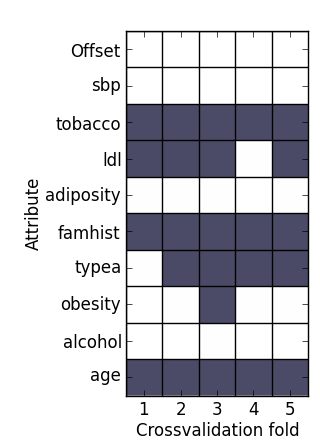
\includegraphics[width=4cm, keepaspectratio=true]{pictures/cv_fold.png}
\caption{Feature selection}
\label{featureSelection}
\end{figure}
From the original list of 9 attributes, only 5 attributes are needed to maintain the performance of the model while making the model more simple. These attributes are:
\begin{itemize}
\item Tobacco
\item ldl
\item famhist
\item typeA
\item Age
\end{itemize}



\subsubsection{Predicting using linear regression}
As of now, the model has an $R^{2}$ of around 0.2 which is not that good. this results in the following prediction from our model:
\begin{figure}[H]
\centering
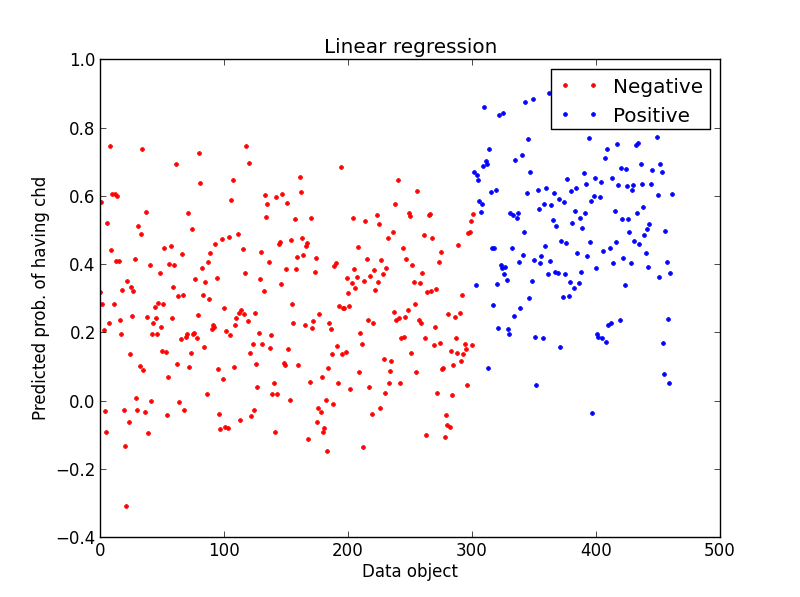
\includegraphics[width=7.5cm, keepaspectratio=true]{pictures/linearPrediction.png}
\caption{Prediction of our linear regression model}
\label{linearPrediction}
\end{figure}
The data is sorted, so it is easier to see the switch from negative CHD to positive.

The plot of the prediction shows that the model is definately not doing an excellent job predicting whether a person has CHD or not, however it is possible too see a pattern, that most negative CHD cases are < 0.5, and most positive CHD cases are > 0.5

The overall misclassification rate using linear regression without feature selection is 35.7\%, and a misclassification rate of 37.1\% with feature selection.

In the following section we will discuss if model transformation could possibly enhance the model
\subsubsection{Residual error plot}
A plot of the residual error vs the attribute shows the following:
\begin{figure}[H]
\centering
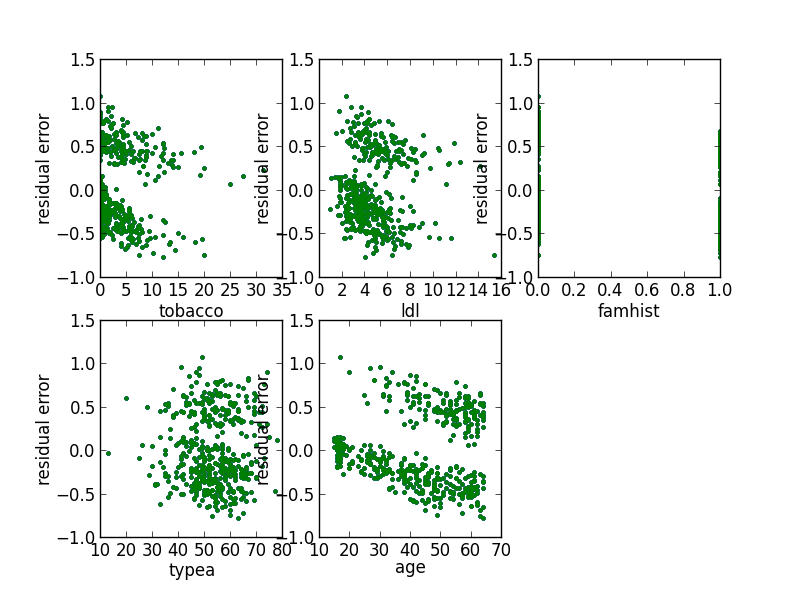
\includegraphics[width=12cm, keepaspectratio=true]{pictures/residual_error.png}
\caption{Plot of residual error vs the attribute}
\label{residualError}
\end{figure}
A good residual error vs attribute plot would be randomly distibuted along the horizontal axis. Looking at the plot, this is not the case for the plotted attributes. This could indicate that a transformation of the attributes could enhance the model.
\subsection{Artificial Neural Network}

When we fit our data to a ANN model with one hidden unit, it had an error rate that kept being around 34\%. This we were able to decrease, by increasing the number of k folds and how many hidden units we had, but this could result in over fitting. Here it would properly be around k folds 10 with 25-50 hidden units maybe it would had been better with more, but because of computation time we could not check those out. This also makes some sense, since we have 462 inputs and the best number of hidden units usually lies between the number of inputs and outputs but if hidden units is placed to high it might overfit.
\\\\
\begin{table}
\begin{longtable}{ccccccc}
\hline 
   & 1 			 & 5 		   & 7 			 & 10		   & 25			 & 50 \\ \hline
5  & 34.623656\% & 34.406265\% & 33.316971\% & 33.328658\% & 30.299205\% & 22.059374\% \\ 
10 & 34.583719\% & 34.204440\% & 34.181314\% & 31.359852\% & 30.083256\% & 21.221092\% \\ \hline 
\end{longtable}
\end{table}
\\
Below you can see the 2 learning curves for 25 and 50 hidden units, with 10 k fold, where you are able to see the numbers of epochs (steps in training process) and how large an error rate were found during the computation.
\begin{figure}[!h]
\centering
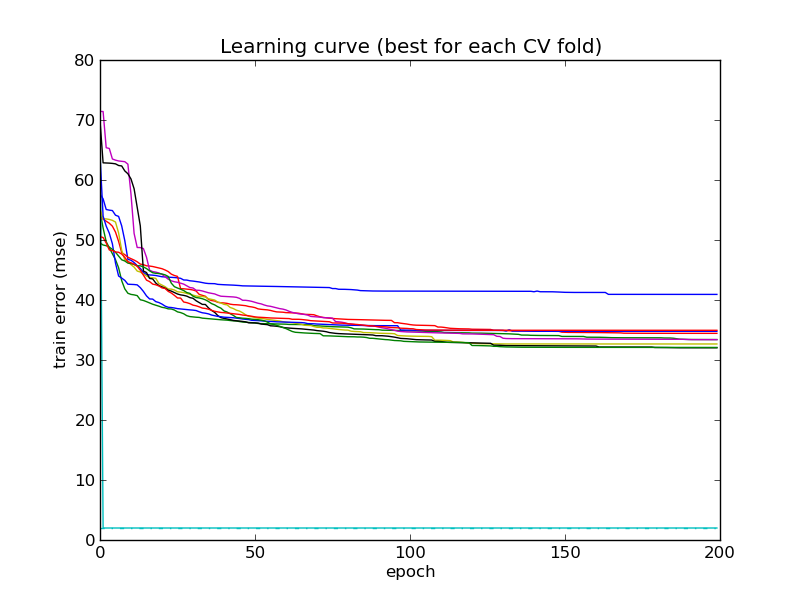
\includegraphics[width=7.5cm, keepaspectratio=true]{pictures/ann_1_10_25.png}
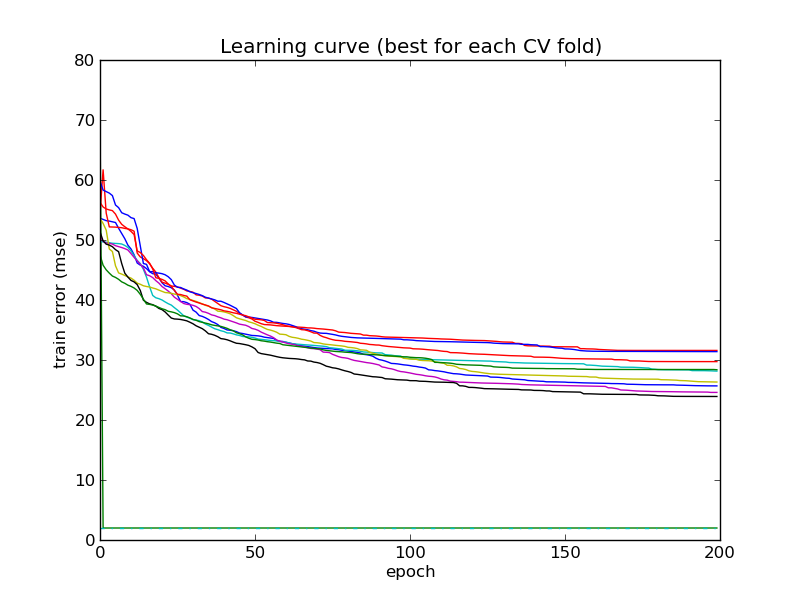
\includegraphics[width=7.5cm, keepaspectratio=true]{pictures/ann_1_10_50.png}
\vspace{-0.4cm}
\caption{\footnotesize 25 hidden vs. 50 hidden on a 10 k fold}
\label{full_10_25_50}
\end{figure}
\\
When we then try to compute the learning curve when we have taken the 4 least important attributes out then we will get something like figure \ref{notfull_10_25_50}. This specific graph has an error rate on 24,25\%, which is a bit higher then the error rate for ANN model for all the attributes. But it is close enough so we can say it shows the same.
\begin{figure}[!h]
\centering
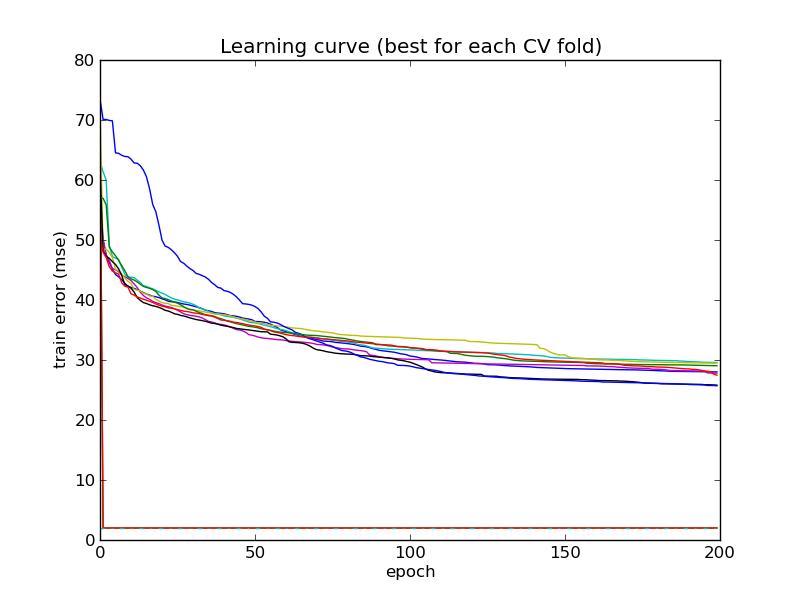
\includegraphics[width=10cm, keepaspectratio=true]{pictures/figure_1.png}
\vspace{-0.4cm}
\caption{\footnotesize 50 hidden on a 10 k fold with the 4 least important attributes taken out}
\label{notfull_10_25_50}
\end{figure}
\newpage
When we then are trying to fit the 2 principle components with the most influence in a ANN model then we are able 2 plot it in a 2d graph, and are able to see how well it actually fit. Since we now have the same numbers of input 462. This time we only have 4 outputs because we needed enough space to fit the output graphs. Figure \ref{ann} shows how well the 2 pc fits with 230 hidden units. You can see in the left lower graph is under fitted since it predict no one to have chd. The other 3 graphs is a bit harder to see if they over, under or just right fitted because of the way our data is structured in the graph. But we could properly say that they are a bit under fitted.
\begin{figure}[!h]
\centering
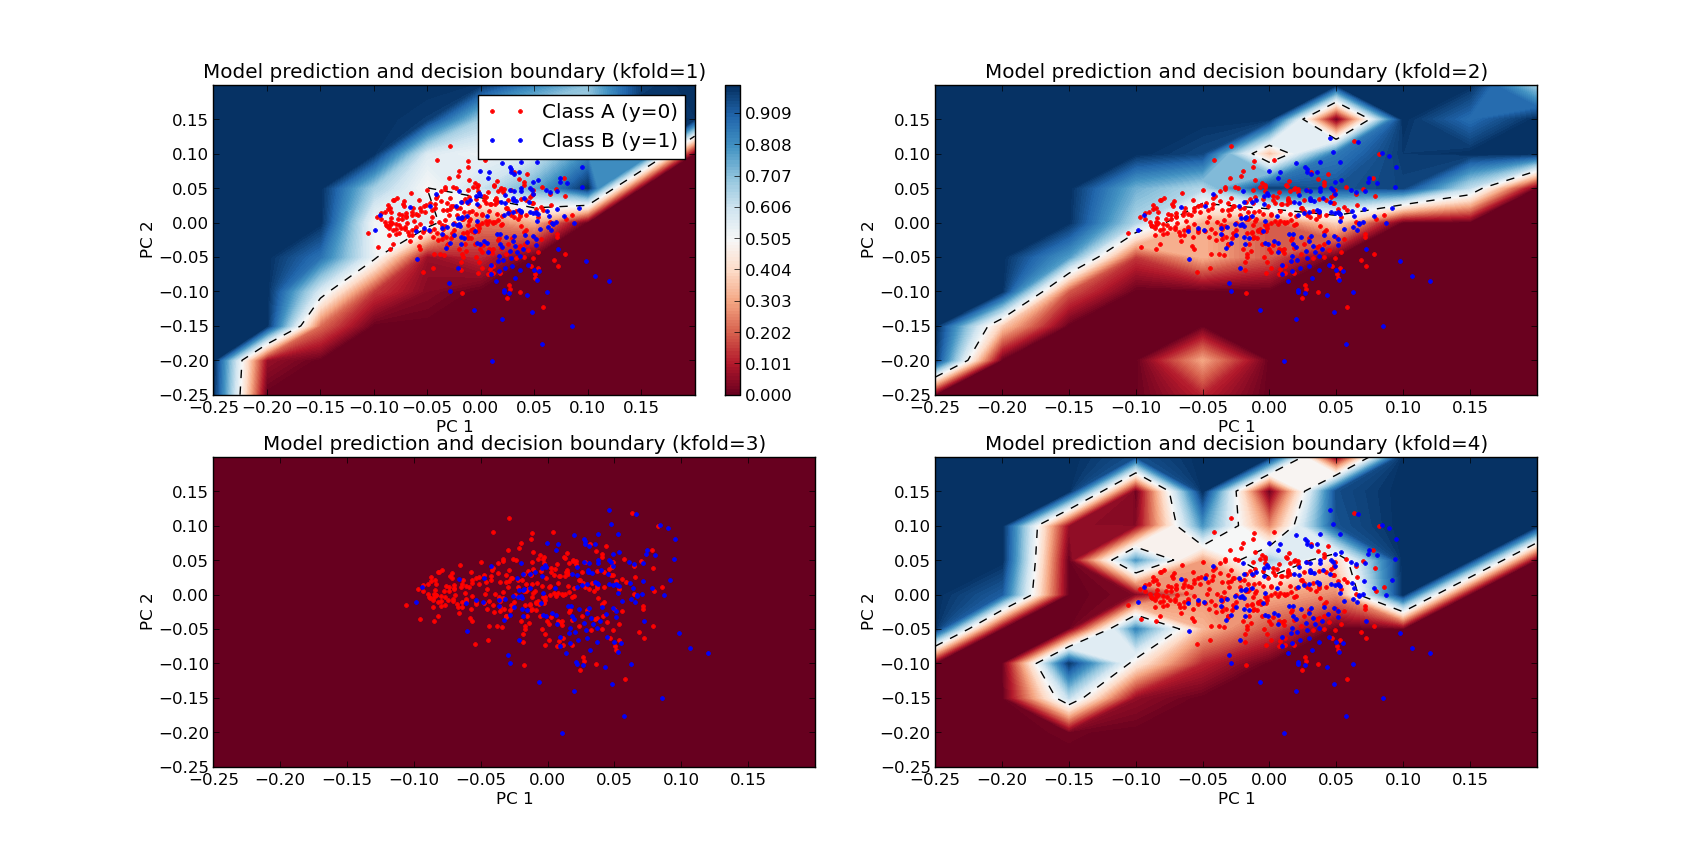
\includegraphics[width=15cm, keepaspectratio=true]{pictures/ann_2_4_230.png}
\vspace{-0.4cm}
\caption{\footnotesize }
\label{ann}
\end{figure}
\\
Figure \ref{ann2} that we see below shows the learning curve of the above figure \ref{ann}, this shows how the training process improved over the number of epochs.
\begin{figure}[!h]
\centering
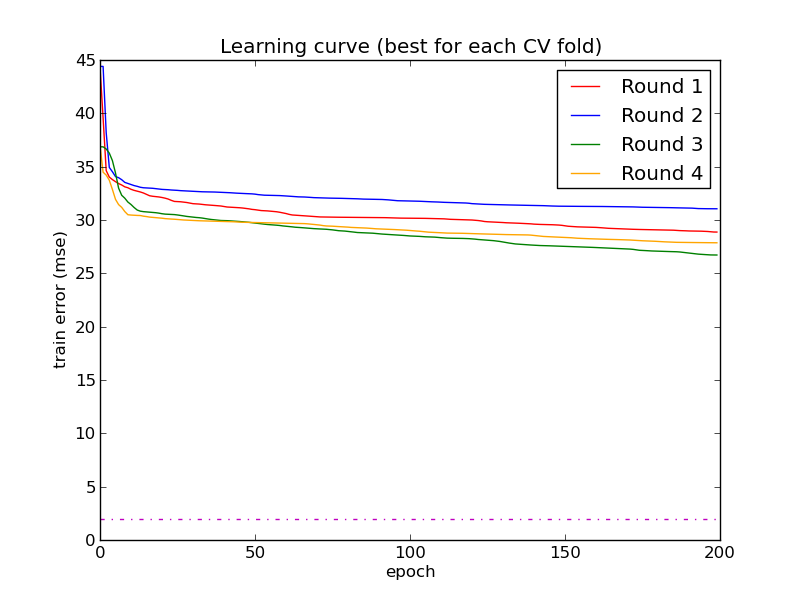
\includegraphics[width=10cm, keepaspectratio=true]{pictures/ann_21_4_230.png}
\vspace{-0.4cm}
\caption{\footnotesize }
\label{ann2}
\end{figure}
\subsection{Comparing regression results}
Comparing the linear regressions misclassification rate, with the artificial neural networks error rate, we get something like this: (Note that fs is: Feature Selection, ANN is "Artificial Neural Network" and the number following ANN defines how many hidden layers are used)
\begin{table}[!h]
\begin{longtable}{lc} \hline
Regression type & error in \% \\ \hline
Linear no fs & 35.7 \\
Linear w/ fs & 37.1\\
ANN 5 & 34.4 \\
ANN 10 & 33.3 \\
ANN 25 & 30.3 \\
ANN 50 & 22.1\\ \hline
\end{longtable}
\end{table}
This shows us that using Artificial Neural Networks seems to be performing better at predicting data in our dataset than Linear regression does. However, even though ANN is performing better than Linear regression, the results are still poor.
%\section{Description}
There is a high level of South Africans with the heart disease \textit{Coronary Heart Disease (CHD)}(?? fodnote). The idea behind the dataset is to see if there is any consistency to why this is a high-risk CHD zone, and to measure what effects the treatment they are given have. The dataset used is a sample of a larger dataset, and consists of 462 rows, containing various information from different persons.

The dataset was described in the South African Medical Journal in 1983, and performed by: \textit{Rossouw JE, Du Plessis JP, Benadé AJ, Jordaan PC, Kotzé JP, Jooste PL, Ferreira JJ}\footnote{http://europepmc.org/abstract/MED/6623218/reload=0;jsessionid=MT3wbNbXg1PKSt1adMMW.10}

We have not been able to recover the journal, as it does not seem to be published on the internet, which means that we do not know what exactly has been done to the data, and what the results of their analysis was.

The sample of the dataset has been obtained from: \textit{http://www-stat.stanford.edu/~tibs/ElemStatLearn/} and is known as: \textit{South African Heart Disease}

\paragraph{We envision that,} after having analyzed the data, we will be able to do a classification of a person, to whether or not he will have CHD. Let us say, we know the systolic blood pressure, tobacco consumption, low density lipoprotein cholesterol, adiposity, history of heart disease in the family, type-a score, obesity, alcohol consumption and age of a given person, then it could be interesting to classify whether or not he is likely to have the disease.%, based on the Principal Component Analysis and correlation between attributes.

Using regression analysis, we can predict some of the attributes, based on the others. So knowing the values of the other attributes, one could be able to calculate the value of another attribute.% I.e given that we know a persons cholesterol number, and his age, we can predict the systolic blood pressure.

Using clustering analysis, we can group persons into categories based on their similarities. This can be done using patterns from our dataset. This could be interesting to see if we have a clustering of subjects, where most of them are sick, or most of them are healthy. If we plot some of the data, it could be interesting if we get for instance a cluster of ill people.

Using association mining, we can discover patterns. For instance, one can check how the presence of heart disease in the family relate to whether the person itself has the disease.% like, if a person is older than 40, and has i high cholesterol number, he might be likely to drink alcohol.

Using anomaly detection, it could be possible to identify outliers in the data. By this we can see if we abnormal data and outliers, the data might be erroneous. Furthermore this might lead to discovering of whether the person is generally healthy. Eg. if he has very high cholesterol or very high tobacco consumption, he might not necessarily have chd, but he might have other health problems.% Based on the pattern from the data, it is possible to see if a reading from the person is out-of-normal, and do something about it.

%Finally the most interesting thing is to be able to classify whether a person has the disease or not based on his systolic blood pressure, tobacco consumption, low density lipoprotein cholesterol, adiposity, history of heart disease in his family, type-a score, obesity, alcohol consumption and age. This is what we have data of for our subjects, and based on the data set one could see if there is any dependency of these and whether a person has the coronary heart disease. Therefore this data set should give an indication of how one can classify the probability of a person having the disease based these attributes.
%\section{Explanation}
In this section we will explain all of the different attributes, our date set contains, as well as how we came to the different types and whether they are discrete or continues attributes. We will also discuss the subject of data issues i.e. missing and corrupted data.

\subsection{Attributes}

\paragraph{Row} is describing the id of the subject. This attribute is \textbf{discrete} and \textbf{nominal}.

\paragraph{SBP} is Systolic blood pressure which is a measurement of the subjects blood pressure, and has the unit mmHg. The desired SBP lies in the range 90-119, but it is plausible to go below or above, but that is when there usually is heart problems.

We came to the type \textbf{interval} because zero as blood pressure is not the lack of pressure, but instead equals 1 atmosphere. Furthermore even though systolic blood pressure normally is described as a real number and therefore as a continuous attribute, for our case we only have natural numbers, meaning the attribute is \textbf{discrete}.%Since we came to interval then the attribute most likely would be \textbf{continues}.

\paragraph{Tobacco} is measured as the cumulative consumption in kg, and since the starting point weight is at 0 kg, and 2 kg is double 1 kg, it would make the attribute type \textbf{ratio}.  The attribute is described as real numbers, it is a \textbf{continuous} attribute.

\paragraph{LDL} stands for Low density lipoprotein cholesterol and is measured in mmol/L. The regular LDL numbers lies around 4.9 mmol/L. It is a \textbf{continuous} attribute, with a \textbf{ratio} type since zero is the absence of LDL and is described by real numbers.

\paragraph{Adiposity} is a sort of indexing for a persons body mass, where this is taken from the waist. It is a \textbf{continuous} attribute since we have real numbers, and it takes on \textbf{ratio} as type. For a man, this value should range from 8\% - 25\% to be in a healthy state, and for a woman it should be 21\% -38\%.

\paragraph{Famhist} short for family history is the attribute that tells if heart disease is present or absent in the persons family, this also make attribute \textbf{discrete} because it is represented as a set of words in the dataset. The type is \textbf{nominal} because it can either be there or not there. We cannot rank the values, we can only put them into categories.

\paragraph{Type-a} is a test score that shows how aggressive a person is. This is a \textbf{discrete} attribute since it is a countable value from 0-100. Because a test score usually is a form of grading system, it would make the type \textbf{ordinal}.

\paragraph{Obesity} Obesity is like adiposity an index for a persons body mass, we better know this one as BMI. It is as adiposity a \textbf{continuous} attribute with the \textbf{ratio} type, since 0 means absence of body mass. This should lie between 18.5 -25 to be within the healthy region of the scale.

\paragraph{Alcohol} is measured as the current alcohol consumption, which we believe is measured as pure alcohol litres consumption over a year. Since we have real numbers and infinitely many possible values, it is a \textbf{continuous} attribute, and because 0 litres of pure alcohol is a absence of what is measured, the type is \textbf{ratio}.

\paragraph{Age} is the age of the subject. It is usually handled as a continues attribute, but in this data set it is treated like a \textbf{discrete} attribute. We have the age in years, meaning we only have the natural numbers. Age has a starting point at 0 which would make it absence of a age and that would make the attribute type \textbf{ratio}.

\paragraph{CHD} stands for coronary heart disease and is a binary attribute that says if the subject has CHD. Since it is binary it makes the attribute \textbf{discrete} and the type would be \textbf{nominal}.

\subsection{Data issues}
As of missing data, we don't really have any corrupted or missing data in any of our data entries, but we do have a single missing data entry at 262. Since it is an entire entry that is missing it will not do any harm to our data models.

Outliers will be covered in section \ref{boxplotSection} concerning boxplots of the attributes.

%\section{Data Visualization}
\subsection{Histogram}
In this section the histograms of the attributes will be covered. In the next section the boxplots for the attributes are explained. The attributes will be explained in details there.
\begin{figure}[H]
\centering
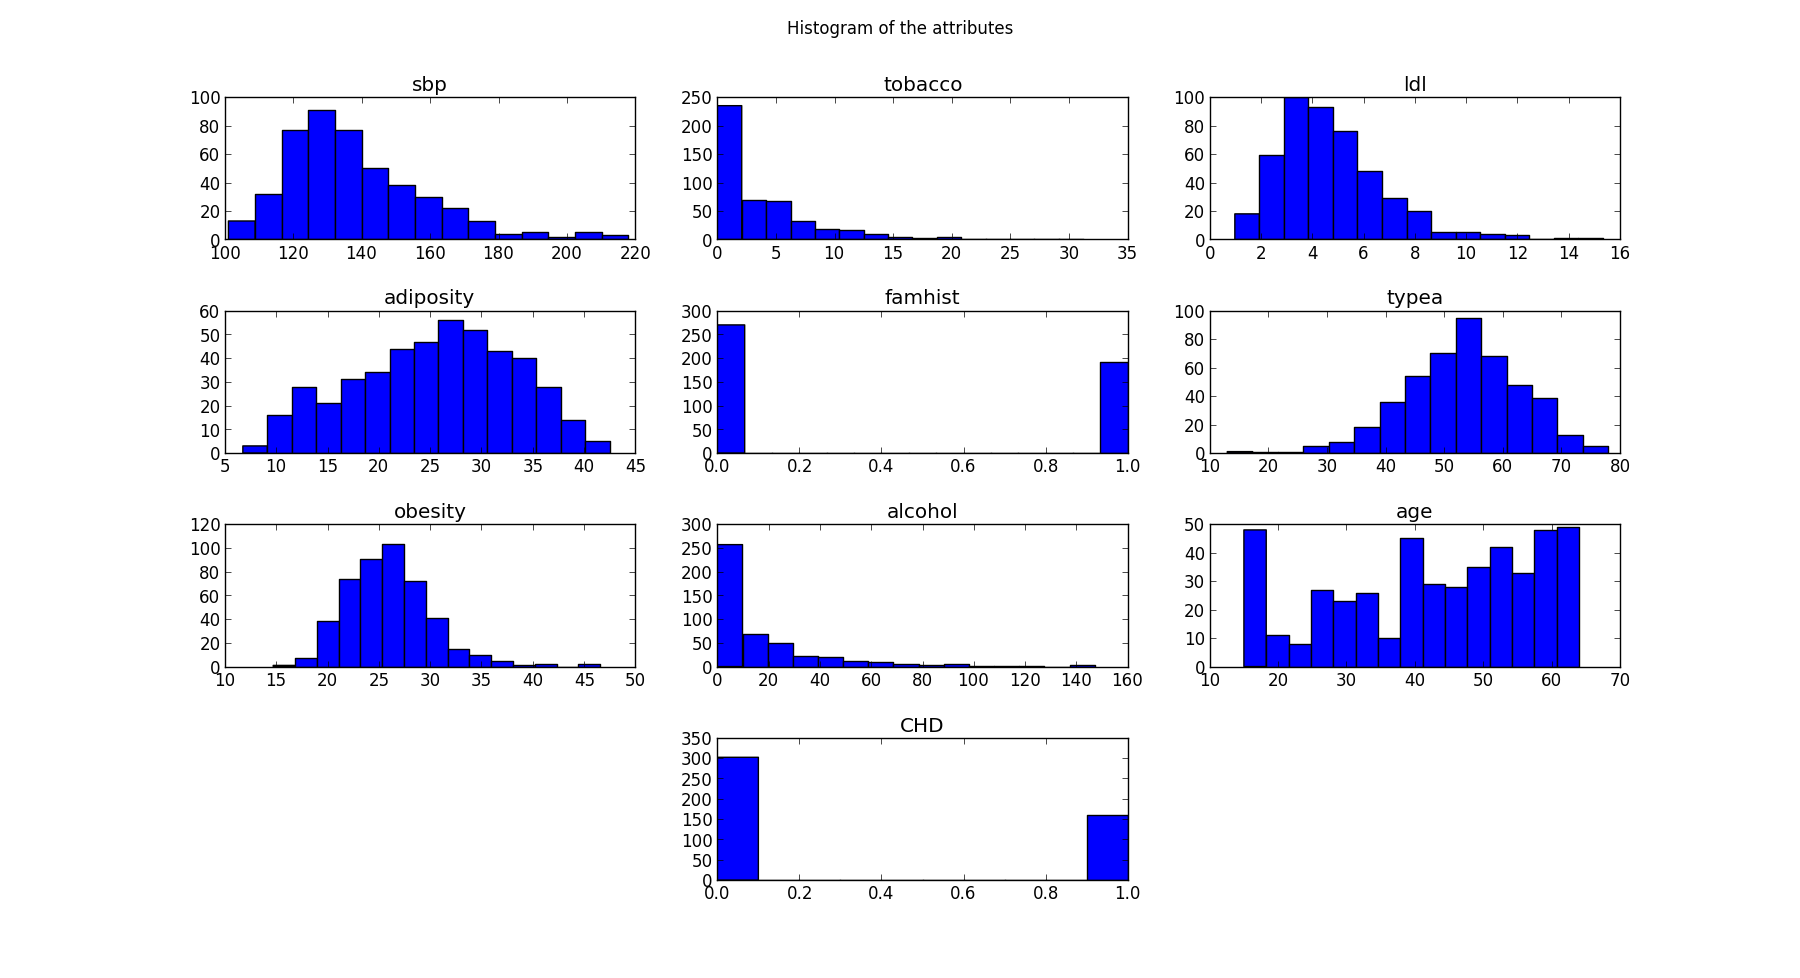
\includegraphics[width=11cm, keepaspectratio=true]{pictures/histogram.png}
\vspace{-0.2cm}
\caption{\footnotesize Histograms}
\vspace{-0.5cm}
\label{histogram}
\end{figure}
Several of our attributes seem to be close to normally distributed. These are listed below:
\paragraph{Adiposity and Obesity} are closely connected, since they both concern the size of the body. How closely connected they are will be explained later.

\paragraph{Type A} is an index of aggresiveness and stresslevel of the person. This is very normally distributed, and peaks at around 55.

\paragraph{SBP - Systolic Blood Pressure} 	seems to be peaking at around 130, which is considered a little bit high, but since the SBP is rising as you get older, and the average age of our dataset is over 40, this seems reasonable. The curve is extending far to the right, which will be covered in section \ref{boxplotSection} about boxplots.

Those attributes not distributed normally are listed below:
\paragraph{Tobacco} indicates that most persons in the dataset does not smoke.
\paragraph{Famhist} Is a binary attribute. Showing a few more people in the dataset does not have any family members with CHD, than who does have family history with CHD.
\paragraph{Alcohol} looks a lot like tobacco. How closely related they are will be considered later.
\paragraph{Age} is ranging from 15 to 65, and shows there are more data from people older than 40.
\paragraph{CHD} is quite important, because this shows us that there are around 300 cases of people \textit{not} having the CHD disease, while only 160 \textit{does} have the disease. This does have an influence in the scatterplots explained later.

\subsubsection{Statistics of the attributes}

Below in Figure \ref{statistics}, one can see the statistics of the attributes.

\begin{figure}[H]
%\section{Statistics of attribute data}

\begin{tabular}{| l | l | l | l | l |}
\hline
 & Mean & Variance & Max & Min \\ \hline
sbp	& 138.33 & 420.10 & 218.0 & 101.0 \\ \hline
tobacco	& 3.64 & 21.10 & 31.20 & 0.0 \\ \hline
ldl	&  4.74 & 4.29 & 15.33 & 0.98 \\ \hline
adiposity & 25.41 & 60.54 & 42.49 & 6.74 \\ \hline
famhist & 0.42 & 0.24 & 1.0 & 0.0 \\ \hline
typea	& 53.10 & 96.38 & 78.0 & 13.0 \\ \hline
obesity & 26.04 & 17.76 & 46.58 & 14.70 \\ \hline
alcohol	& 17.04 & 599.32 & 147.19 & 0.0 \\ \hline
age	& 42.82 & 213.42 & 64.0 & 15.0 \\ \hline
\end{tabular}

\caption{Showing the mean, variance, maximum and minimum for the attributes.}
\label{statistics}
\end{figure}
\subsection{Boxplots}
In the following section we will discuss what the boxplots of the attributes tell us about the data.
Below is a figure representing the boxplot for the referenced attribute.
\begin{figure}[H]
\centering
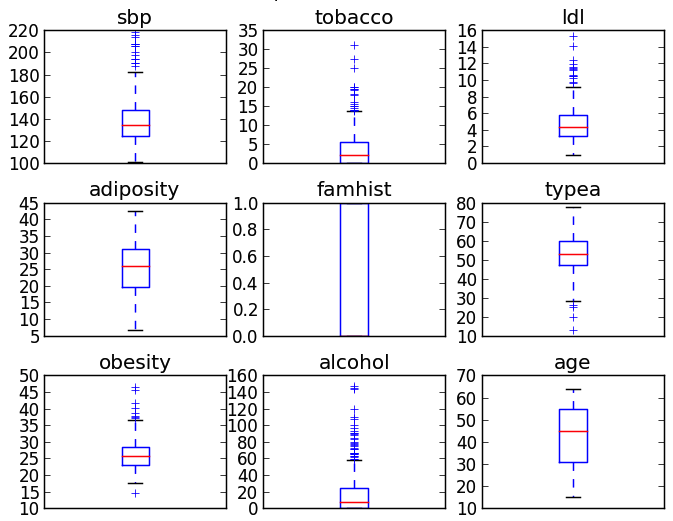
\includegraphics[width=12cm, keepaspectratio=true]{pictures/boxplot.png}
\caption{\footnotesize Boxplots}
\label{boxplot}
\end{figure}
\paragraph{SBP - Systolic Blood Pressure} shows us that most of the measured blood pressure is close to 130 mmHg. However, we see that there is some outliers in the dataset. This raises some suspicion to the readings. According to other sources \footnote{http://en.wikipedia.org/wiki/Blood\_pressure}, when the blood pressure rises above 180 mmHg for a longer period of time, organs will start to fail. This could indicate that some of the data are incorrect.

In total there are 15/462 outliers in this attribute.

\paragraph{Tobacco consumption} is another boxplot which is showing a large amount of outliers in the data. This time however, it is not necessarily bad data, but just a higher level of use. Since it is based on the total amount of tobacco in kilos, used over the persons life time, it is expected to see some very high values at people who started smoking early, and is older than the average.

\paragraph{ldl - low density lipoprotein cholesterol} is measured in mmol/L. Anything above 4.9 is considered a high cholesterol \footnote{http://www.mayoclinic.com/health/cholesterol-levels/CL00001}. This seems to be consistent with the data from the boxplot. But again there are some outliers, and it does seem odd to have an ldl value more than tripple what is considered to be high.

In total there are 14/462 outliers in this attribute.

\paragraph{Adiposity - BAI} is an index number to group people by their size, much like BMI. The boxplot shows no outliers, and the average is consistent with what is considered to be normal. \footnote{http://easycalculation.com/health/body-adiposity-index.php}

\paragraph{Famhist} is a binary value, and does not tell us anything useful in a boxplot. Off to the next attribute.

\paragraph{TypeA} is an indicator to show aggresiveness of a person, based on an evaluation. Even though there are outliers in the boxplot, we do not consider those as suspicious, as the index ranges from 0 to 100.

\paragraph{Obesity - BMI} is another indicator of the persons size, much like the adiposity index, just calculated a bit different. Since the adiposity and BMI index is closely correlated (as shown later) we do not consider the outliers to be a concern. The outliers do still lie within a plausible BMI value.

\paragraph{Alcohol} contains a lot of outliers. Most of the readings from the dataset shows an alcohol consumption of 0, or nearly 0, which makes the average consumption almost 0. It is well known, that some have a considerably higher alcohol consumption level than average, however, because of the amount of outliers, and the much higher readings on some of the persons, this is a little suspicious.

In total there are 33/462 outliers in this attribute.

\paragraph{Age} does not show us any really useful in a boxplot, except for the fact that the age range goes from around 15 to 65.

\paragraph{Summary:} Because of the amount of outliers in the dataset, especially SBP, ldl and alcohol, there are some uncertainty regarding the reliability of the data.


\section{Comparing Attributes}
To be able see if any of the attributes have had an big effect on whether the different subjects got CHD, we plotted some of the attributes against he each other, this would also help us to spot highly unlikely data.

\subsection{Tobacco vs. Alcohol}

Some of the attributes we thought would be interesting to compare to each other, were amongst other tobacco and alcohol, since these are often considered bad for peoples health. In figure \ref{AlcoTobac} we can see those two attributes plotted against each other. Here it does look like that tobacco has an bigger influence on CHD the alcohol, but we cannot tell that much more about these two from this figure since the spread of negative and positive seems very similar. However it seems like people located in the extremes, meaning smoking and drinking a lot, are more exposed to the disease.

\begin{figure}[H]
\centering
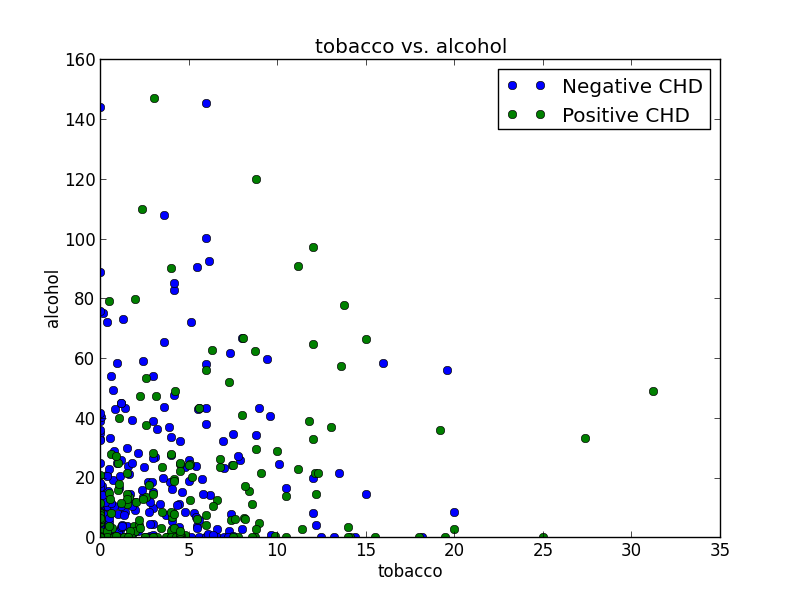
\includegraphics[width=7cm, keepaspectratio=true]{pictures/tobaccoAlcohol.png}
\vspace{-0.4cm}
\caption{\footnotesize Tobacco vs. Alcohol}
\label{AlcoTobac}
\end{figure}

\subsection{Obesity vs. Adiposity}

Alcohol and tobacco wasn't the only attribute we thought would be interesting to look at, we also thought of what the more obese subject would look like. In the comparison figure \ref{ObeAsi} we see the adiposity and obesity put up against each other. First of all, we see that the two attributes depend quite much at each other, which we would also expect. The tendency of the graph is that the higher adiposity, the higher obesity. However something that catches your eyes in this, is the top left dot and the bottom right dot. These two is a bit different than the others, since they lie far from mass of subject that gathers in a bit bend line. This could be the result of wrongful data or just a bit bizarre subject. But these would be considered outliers in this comparison.

When you look at figure \ref{ObeAsi} you see the that the higher the values get the more subjects got CHD. This could say that the higher numbers a subject got in adiposity and obesity the chance there is for the subject to get CHD.

\begin{figure}[H]
\centering
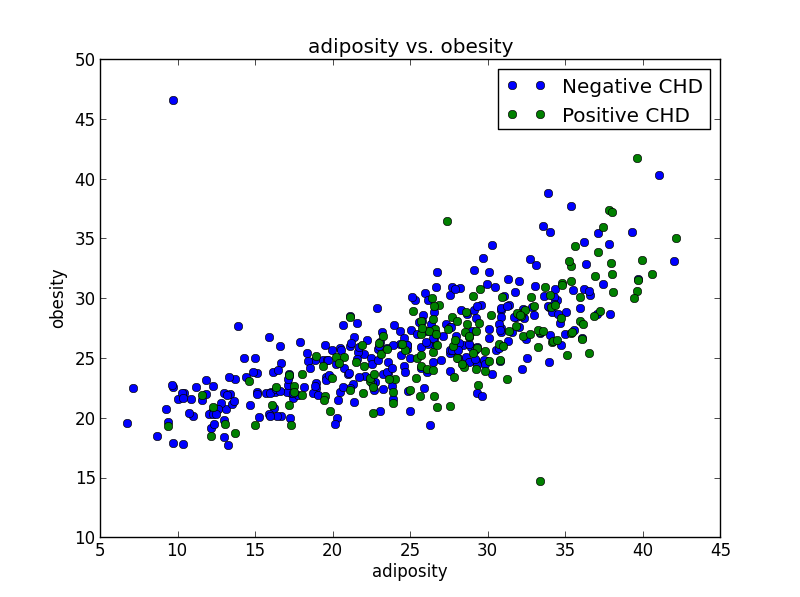
\includegraphics[width=7cm, keepaspectratio=true]{pictures/adiposityObesity.png}
\vspace{-0.4cm}
\caption{\footnotesize Adiposity vs. Obesity}
\label{ObeAsi}
\end{figure}

\subsection{Type-a vs. Alcohol}

In figure \ref{typeAlco} we try to see if more aggressive subjects have a higher chance on getting CHD, and if alcohol would make difference in how aggressive subject would be. What we can see in the figure is at first that alcohol does not seem to have a big influence on how aggressive the different subjects are. But it does seem the very aggressive people have an higher chance of being positive for CHD. In general it seems like there is a similar spread in both positive and negative tested subjects.

\begin{figure}[H]
\centering
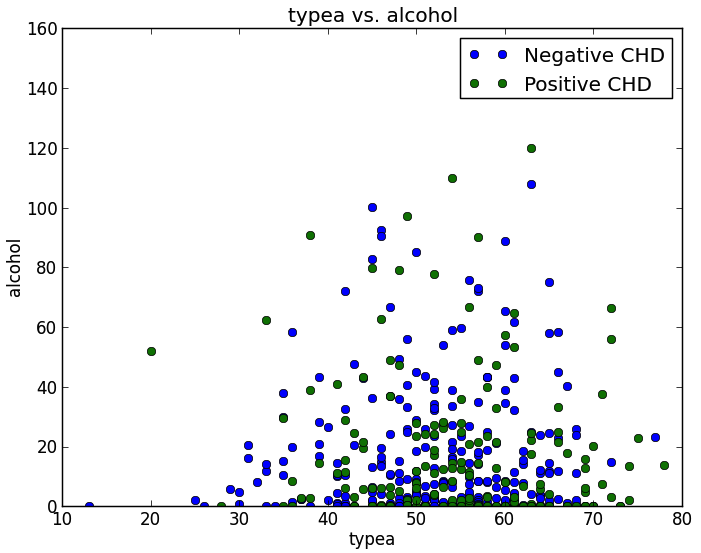
\includegraphics[width=7cm, keepaspectratio=true]{pictures/typeaalcohol.png}
\vspace{-0.4cm}
\caption{\footnotesize Type-a vs. Alcohol}
\label{typeAlco}
\end{figure}
\subsection{Principal Component Analysis}

\subsubsection{Variance explained by Principal Components}

In Figure \ref{VariancePCA}, we can see how the variance is explained by the principal component. We can see that the first principal component explains 32\% of the variance, while the second component explains 13\% of the variance. This means that we can explain 45\% of the total variance by using the two first principal components. Furthermore one can see from the graph that we need 5 principal components in order to explain 75\% of the variance, and at least 7 components to explain 90\% of the variance.

\begin{figure}[H]
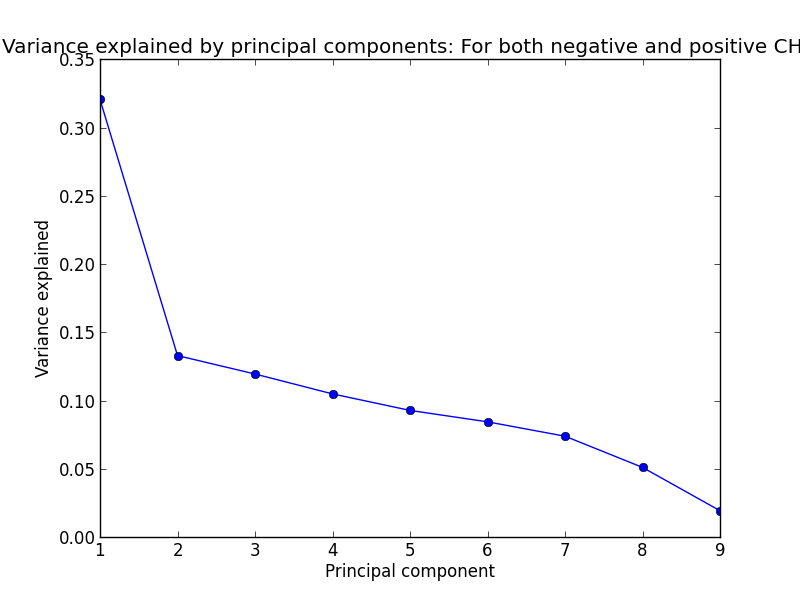
\includegraphics[scale=0.75]{pictures/PCAPosAndNeg.png}
\caption{Showing how the variance is explained by the principal components.}
\label{VariancePCA}
\end{figure}

\subsubsection{Direction of the principal components}

Below in Figure \ref{PCADirections}, we can see the directions of the principal components. The most interesting components are the first ones, as these describe the biggest part of the variance. Looking at the first principal component, we see that obesity, adiposity and age are very relevant, while the second principal component is mostly (??: Bad word to use?) described by alcohol and tobacco. We see that all the attributes effect the principal components, meaning they all have impact, however some attributes have larger impact than others. Eg. typea and family history are not heavily described by the first two principal components.

\begin{figure}[H]
\begin{longtable}{ l c c c c c c c c c}
 \hline
 \emph{Attributes} &  \emph{sbp} &  \emph{tobacco} &  \emph{ldl} & \emph{adiposity} &  \emph{famhist} &  \emph{typea} &  \emph{obesity} &  \emph{alcohol} &  \emph{age} \\ \hline
PC1 & -0.3238 & -0.3018 &  -0.3339 &  -0.5163 & -0.1951 & 0.0183 & -0.4015 & -0.1214 & -0.4601 \\ 
PC2 & 0.2383 &  0.4585 & -0.3639 &  -0.1876 &  0.0013 &   -0.2822 & -0.3919 & 0.5430 & 0.1930 \\ 
PC3 & -0.1251 & 0.0682 &  0.0031 & -0.0819 &  0.3384 & 0.7923 & 0.0402 &  0.4591 & -0.1353 \\ 
PC4 & -0.1964 & 0.0054 & 0.1403 & -0.1350 &  0.8334 & -0.2098 & -0.3055 & -0.2585 &  0.1573 \\ 
PC5 & 0.2149 & -0.6236 & -0.2422 &  0.1189 &  0.3054 & -0.3210 & 0.2834 &  0.4190 &  -0.1999 \\ 
PC6 & -0.7814 &  0.1631 &   0.2153 &  0.1309 & -0.0857 & -0.3319 & 0.1736 & 0.3793 & -0.0887 \\ 
PC7 & -0.2681 &  0.1929 & -0.7882 &  0.1957 &  0.1285 &  0.0778 & 0.3333 & -0.2768 &  0.1453 \\ 
PC8 & 0.2354 &  0.4889 &  0.0703 & -0.1731 & 0.1866 & -0.1655 &   0.3387 & -0.1251 & -0.6914 \\ 
PC9 & -0.0141 & -0.0478 & 0.0719 & -0.7575 & -0.0288 & -0.0406 & 0.5040 & 0.0331 & 0.4012 \\ \hline  
\end{longtable}
\caption{Describing the directions of the principal components.}
\label{PCADirections}
\end{figure}

\subsubsection{Projection of data onto Principal Components}

We can see the data projected onto the first two principal components in Figure \ref{PCAProjected}. At first glance it is hard to see a pattern. However one can see that most of the sick people are located in a direction, where the first principal component is negative. By comparing to how the attributes are described in this component, as shown in Figure \ref{PCADirections}, we see that this principal component are pointing in the negative direction for all the attributes, except typea which is hardly described in this component. And since we have a lot of ill subjects in this negative direction of principal component 1, it indicates that these people have high values in these attributes. Meaning these subjects have a tendency to have high adiposity for instance. The data has been standardized for doing this principal component analysis, meaning that Figure \ref{PCAProjected} indicates that many of the ill subjects has values above the mean in most attributes.

\begin{figure}[H]
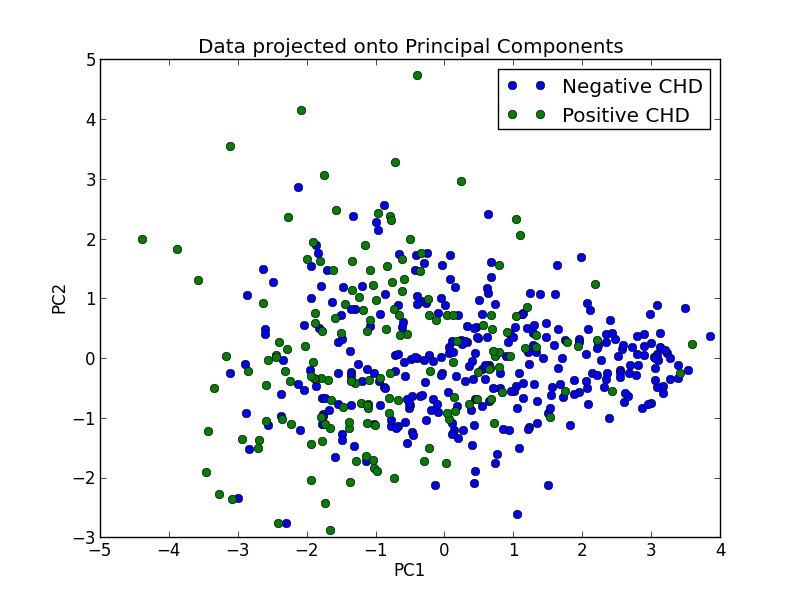
\includegraphics[scale=0.75]{pictures/projectedToPCA.png}
\caption{Projection of data onto first two principal components.}
\label{PCAProjected}
\end{figure}

\section{Correlation of the data}

Below in Figure \ref{correlationTable}, we see how the attributes are related to each other. For instance, we can see that obesity is highly related to adiposity, however the most interesting thing is to see how the attributes might have an impact on whether the subject has the disease or not. So the correlations to chd are the most interesting to look at.

\begin{figure}[H]
\begin{tabular}{ | l | l | l | l | l | l | l | l | l | l | l | }
  \hline                        
  Correlation & sbp & tobacco & ldl & adiposity & famhist & typea & obesity & alcohol & age & chd	\\ \hline
sbp & 1 & 0.2122 & 0.1583 & 0.3565 &  0.0856 & -0.0575 &
   0.2381 & 0.1401 &  0.3888 & 0.1924 \\ \hline
   
 tobacco & 0.2122 & 1 & 0.1589 &  0.2866 &  0.0886 & -0.0146 &
   0.1245 &  0.2008 & 0.4503 &  0.2997 \\ \hline
   
ldl & 0.1583 & 0.1589 &  1 &          0.4404 &  0.1613 &  0.0440 &
   0.3305 &  -0.0334 &   0.3118 & 0.2630 \\ \hline

adiposity &  0.3565 & 0.2866 & 0.4404 & 1 &          0.1817 & -0.0431
 &  0.7166 &  0.1003 &  0.6260 & 0.2541 \\ \hline

famhist & 0.0856 & 0.0886 &  0.1614 &  0.1817 &  1      &    0.0448 &
   0.1156 & 0.0805 &  0.2397 &  0.2724 \\ \hline

typea & -0.0575 & -0.0146 &  0.0440 & -0.0431 &  0.0448 &  1 &
   0.0740 &   0.0395 & -0.1026 &  0.1032 \\ \hline

obesity & 0.2381 &  0.1245 &  0.3305 &  0.7166 &  0.1156 &  0.0740 &
   1 &          0.0516 &  0.2918 &  0.1001 \\ \hline

alcohol & 0.1401 & 0.2008 & -0.0334 &   0.1003 &  0.0805 &  0.0395 &
   0.0516 &  1 &          0.1011 &  0.0625 \\ \hline

age & 0.3888 &  0.4503 &  0.3118 &  0.6260 & 0.2397 & -0.1026 &
   0.2918 &  0.1011 &  1     &     0.3730  \\ \hline
  
  
chd &  0.1924 & 0.2997 & 0.2631 & 0.2541 & 0.2723 & 0.1032 & 0.1001 & 0.0625 & 0.3730 & 1 \\ \hline
\end{tabular}
\caption{Table showing how the attributes are correlated to whether subjects have positive or negative chd.}
\label{correlationTable}
\end{figure}

We see that the CHD attribute is not totally dependent on any of the other attributes, but the attribute with the most impact is the age. On the other hand we see that alcohol has the smallest correlation to CHD. So this indicates that age has greater influence compared to alcohol, when to get the possibility of a man having the disease. In fact this table shows that the alcohol consumption has very small meaning for whether a person has the disease.
%\section{Discussion}
The dataset leaves us with some concern to whether or not all of the attributes are actually right. As described in the boxplot section with the outliers, there are several of these, and some of them could indicate problems with some of the data


\section{Classification}
\label{classification}
For our classification, we have worked with Logistic Regression, Decision Tree and K-nearest neighbours. All these methods have been applied, where we look at all the attributes of our dataset, where we only look at the attributes with the most importance according to our forward selection section \ref{ForwardSelection}, where we have standardized the data according to find principal components looking at all the principal components, and where we only look at the two most important principal components. Meaning we have given our data as four different types of input for these methods.

\subsection{Logistic Regression}

We have applied logistic regression to our data. For logistic regression, we calculate a value for each data object. This value can be used to estimate the likelihood of the object to be CHD positive.

\begin{figure}
	\begin{subfigure}[b]{0.5\textwidth}
	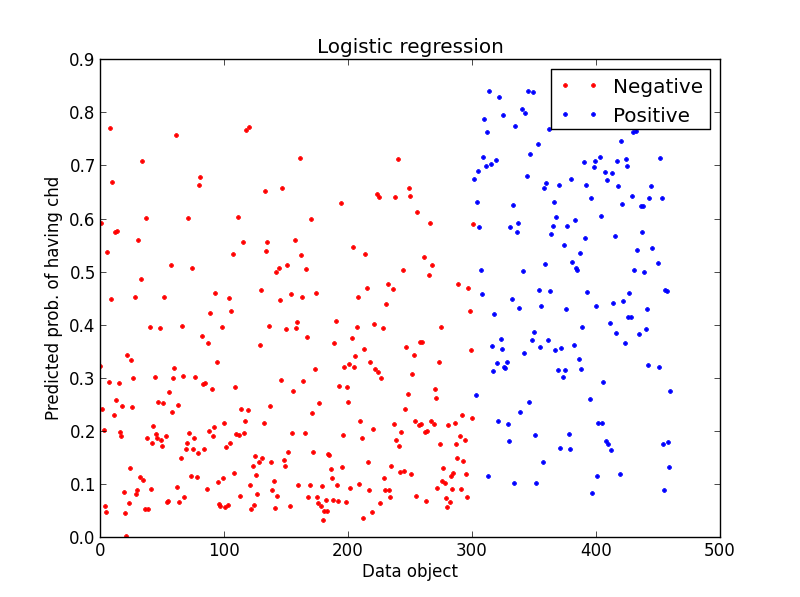
\includegraphics[scale=0.4]{pictures/logisticregressionX.png}
	\caption{Looking at all attributes.}
	\label{logicalRegressionResultX}
	\end{subfigure}
	\begin{subfigure}[b]{0.5\textwidth}
	\includegraphics[scale=0.4]{pictures/logisticregressionXad.png}	
	\caption{Looking at attributes selected by forward selection.}
	\label{logicalRegressionResultXad}
	\end{subfigure}

	\begin{subfigure}[b]{0.5\textwidth}
	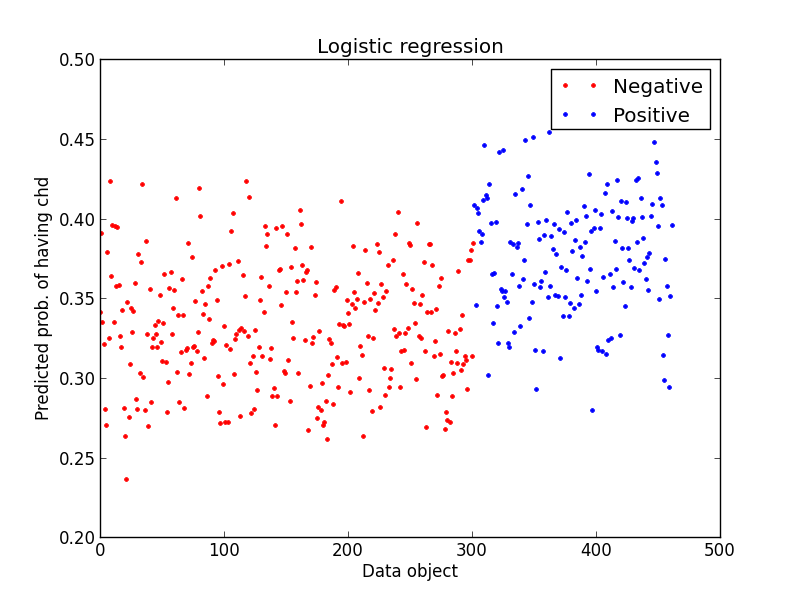
\includegraphics[scale=0.4]{pictures/logisticregressionXPC.png}
	\caption{Looking at all principal components.}
	\label{logicalRegressionResultXPA}
	\end{subfigure}
	\begin{subfigure}[b]{0.5\textwidth}
	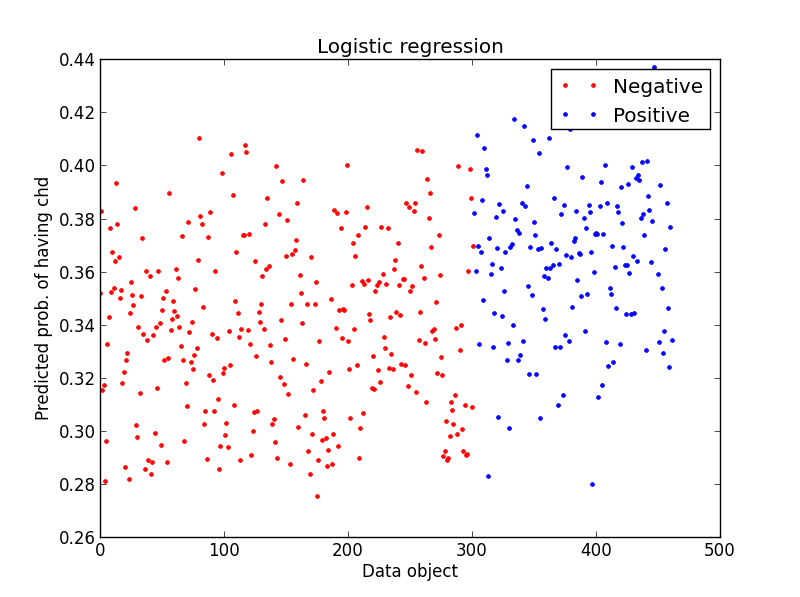
\includegraphics[scale=0.4]{pictures/logisticregressionX2PC.png}
	\caption{Looking at two most important principal components.}
	\label{logicalRegressionResultX2PA}
	\end{subfigure}
\caption{This figure shows results of performing logical regression for different input.}
\label{logicalRegressionResults}
\end{figure}

Se Figure \ref{logicalRegressionResults} to see output for our different input, when running Logistic Regression. Looking at Figure \ref{logicalRegressionResultX}, we see our results, when we have not alternated with the data, and likewise we see at Figure \ref{logicalRegressionResultXad}, our results for when, we have removed the attributes with less influence, meaning for this case we only look at the attributes: Age, Alcohol, Type-A, Family history, Low density lipoprotein cholesterol (LDL). For see especially from these to output of results that there is a tendency for subjects actually having the disease to have a higher probability of having the disease, even though we still see subjects having the disease with low predicted probability and likewise subjects not having the disease having a high predicted probability.

Looking at Figures \ref{logicalRegressionResultXPA} and \ref{logicalRegressionResultX2PA}, where we use principal components to give a logical regression of the data, also see a tendency of people actually having the disease, also have a higher predicted probability of having the disease. However we see that the interval of predicted probabilities are much less. Actually we see from these two graphs that all subjects have a predicted probability of less than 50\%.

A naive way of classifying subjects from these results, is classifying subjects with a predicted probability of more than 50\% as CHD-positive and vice versa the rest as being CHD-negative. This way we can go through all the subjects of the sets, and see how big a percentage are classified correct or wrong. This gives us the misclassification rate. These can be seen in Figure \ref{logicalRegressionErrorRate}

\begin{table}
\begin{longtable}{lc} \hline
Result from: & Mis-classification rate \\ \hline
Figure \ref{logicalRegressionResultX} & 26,6\% \\ 
Figure \ref{logicalRegressionResultXad} & 25,8\% \\ 
Figure \ref{logicalRegressionResultXPA} & 34,6\% \\ 
Figure \ref{logicalRegressionResultX2PA} & 34,6\% \\ \hline
\end{longtable}
\caption{Mis-classification rate for the logistic regressions.}
\label{logicalRegressionErrorRate}
\end{table}

We see that we actually get the smallest misclassification rate, when we look at the results from when we do not use principal component analysis, but we also see that in this case, we can use the results from our forward selection to decrease the misclassification result. For comparing these misclassification rates, we should compare to just classifying all objects to be negative. For this we get a misclassification rate of $\frac{160}{462}=34,6\%$, as we have 160 positive samples from a total of 462 samples. We see that this misclassification rate corresponds to the results described in Figures \ref{logicalRegressionResultXPA} and \ref{logicalRegressionResultX2PA}. This makes sense, since the predicted probability of all subjects in these cases are below 50\%.

\input{decisionTree}

\subsection{K-nearest neighbours}

The data set has been exposed to classification by looking at the k nearest neighbours.

\begin{figure}
	\begin{subfigure}[b]{0.5\textwidth}
	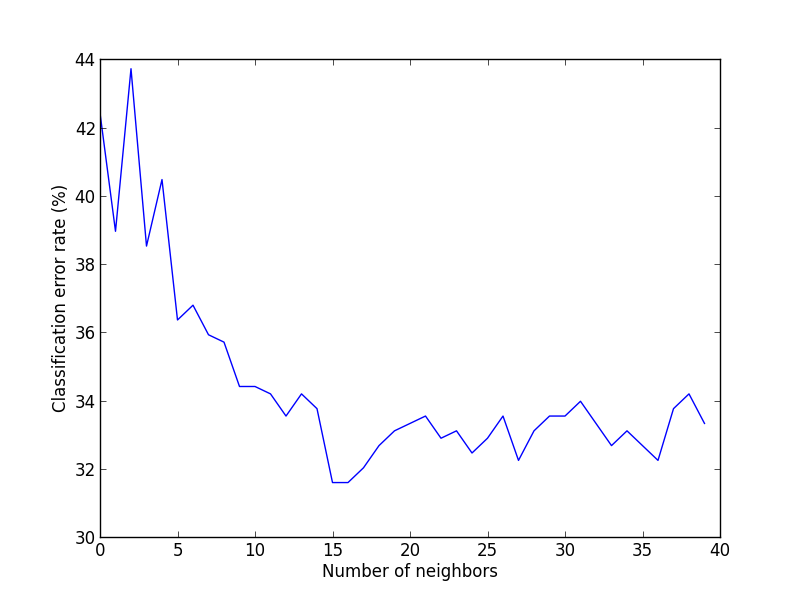
\includegraphics[scale=0.4]{pictures/knnX.png}
	\caption{Looking at all attributes.}
	\label{logicalRegressionResultX}
	\end{subfigure}
	\begin{subfigure}[b]{0.5\textwidth}
	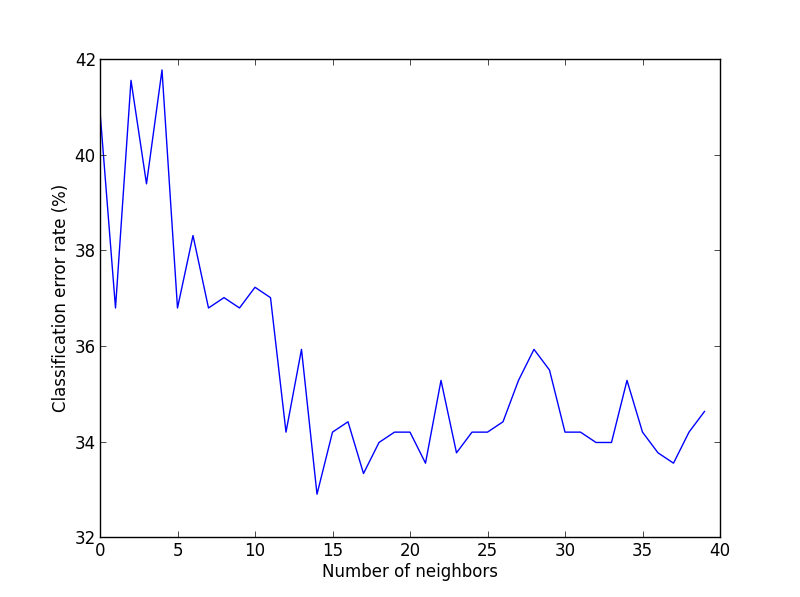
\includegraphics[scale=0.4]{pictures/knnXAD.png}	
	\caption{Looking at attributes selected by forward selection.}
	\label{logicalRegressionResultXad}
	\end{subfigure}

	\begin{subfigure}[b]{0.5\textwidth}
	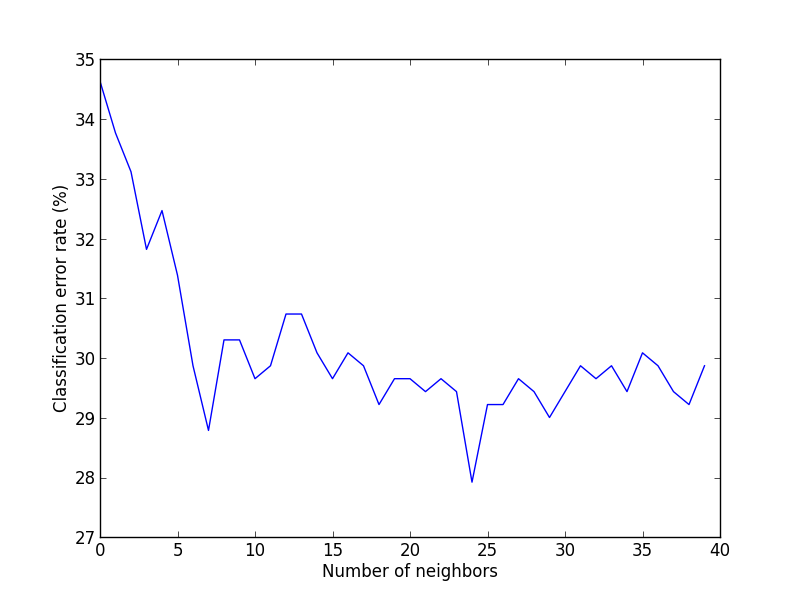
\includegraphics[scale=0.4]{pictures/knnPC.png}
	\caption{Looking at all principal components.}
	\label{logicalRegressionResultXPA}
	\end{subfigure}
	\begin{subfigure}[b]{0.5\textwidth}
	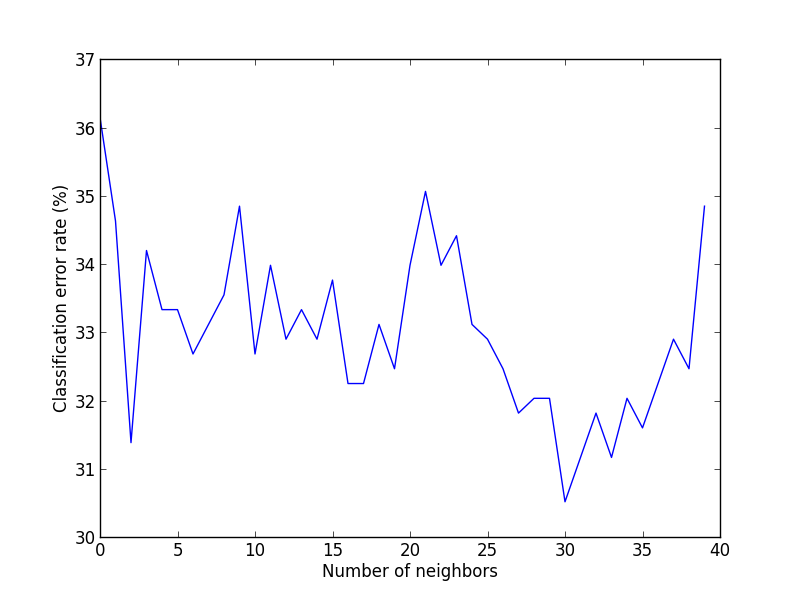
\includegraphics[scale=0.4]{pictures/knn2PC.png}
	\caption{Looking at two most important principal components.}
	\label{logicalRegressionResultX2PA}
	\end{subfigure}
\caption{This figure shows results of performing logical regression for different input.}
\label{logicalRegressionResults}
\end{figure}


\begin{figure}
	\begin{subfigure}[b]{0.5\textwidth}
	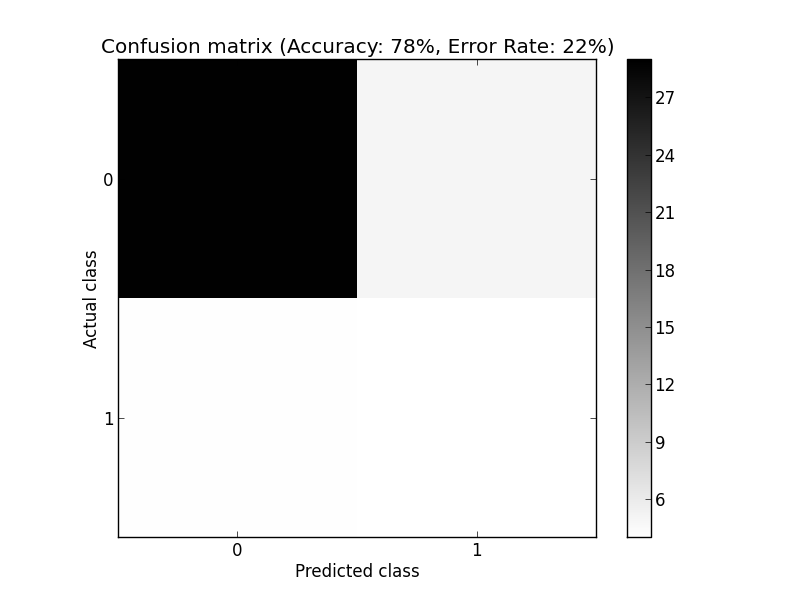
\includegraphics[scale=0.4]{pictures/cmX.png}
	\caption{Looking at all attributes.}
	\label{logicalRegressionResultX}
	\end{subfigure}
	\begin{subfigure}[b]{0.5\textwidth}
	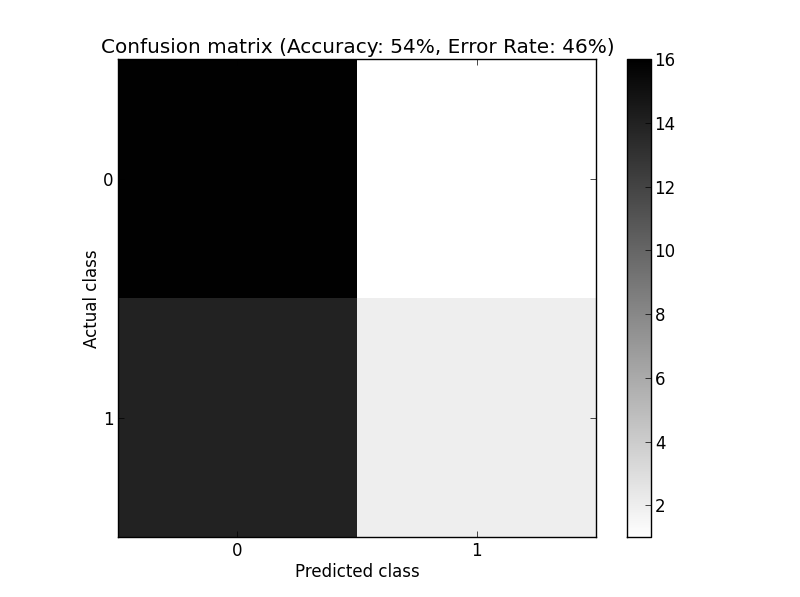
\includegraphics[scale=0.4]{pictures/cmXAD.png}	
	\caption{Looking at attributes selected by forward selection.}
	\label{logicalRegressionResultXad}
	\end{subfigure}

	\begin{subfigure}[b]{0.5\textwidth}
	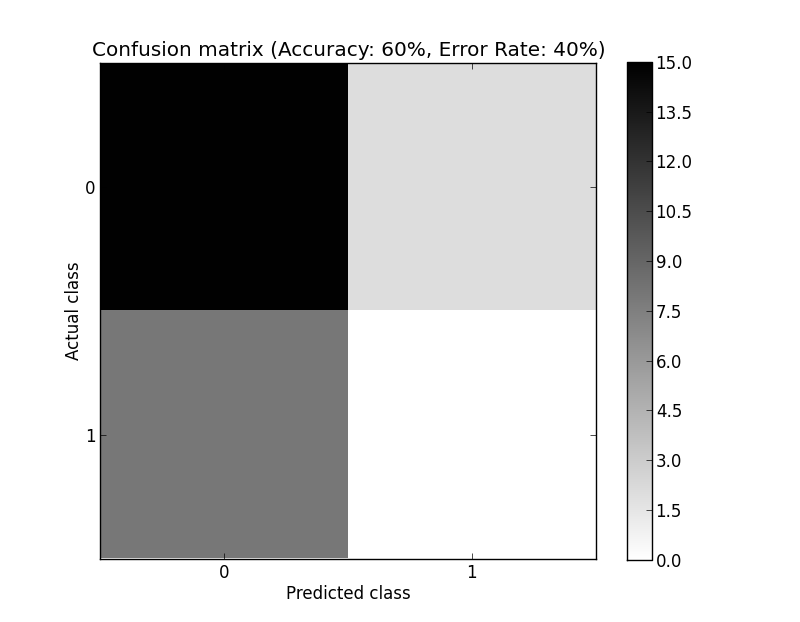
\includegraphics[scale=0.4]{pictures/cmPC.png}
	\caption{Looking at all principal components.}
	\label{logicalRegressionResultXPA}
	\end{subfigure}
	\begin{subfigure}[b]{0.5\textwidth}
	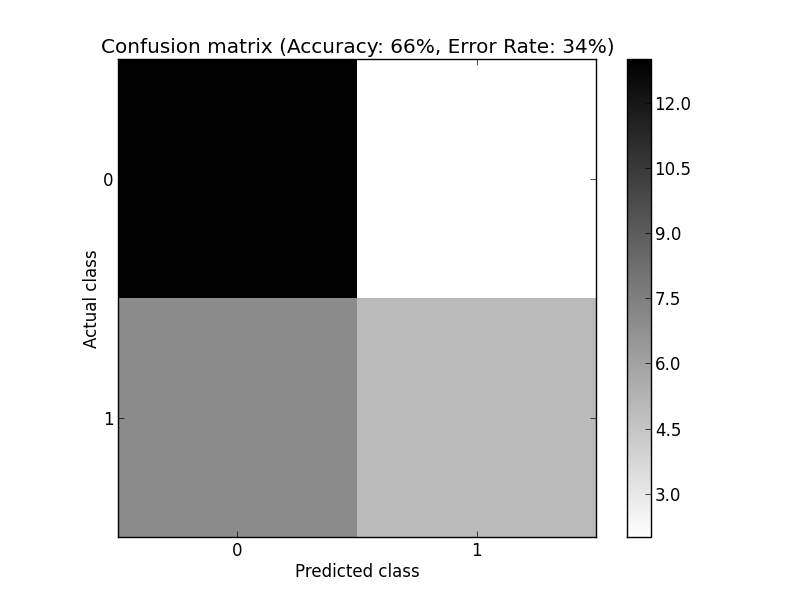
\includegraphics[scale=0.4]{pictures/cm2PC.png}
	\caption{Looking at two most important principal components.}
	\label{logicalRegressionResultX2PA}
	\end{subfigure}
\caption{This figure shows results of performing logical regression for different input.}
\label{logicalRegressionResults}
\end{figure}



We have compared the tree methods of classification with each other. For each method, we have looked at and calculated the misclassification rate, as described in sections (??TODO REF). However here we use the whole data set to describe the classification. And we then check the misclassification rate using the same data objects. Therefore we have also for these 3 approaches created random train and test sets. So we use a subset of our data set to train a classifier, and then we use another subset of the data set to estimate the misclassification. We have done this for 5 randomly generated sets. The results of this can be seen in \ref{misclasRes}. This figure indicates that Logical Regression (LR) is not very suitable for our data set. We also see that the misclassification results of Section (??TODO Ref) are quiet different from these. The table for instance shows us that Decision Trees might be better than eg. Logical Regression for our set.

\begin{table}
\begin{tabular}{|l|l|l|l|l|l|l|}
\hline
Method & test1 & test2 & test3 & test4 & test5 & Mean \\ \hline
LR / All attributes & 0.4792 & 0.2917 & 0.5 &   0.375 & 0.3333 & 0.3958\\ \hline
LR / According to FF & 0.3333 & 0.5208 & 0.4375 & 0.3125  &  0.3958 & 0.4    \\ \hline
LR / Principal Components & 0.4375  &  0.3333 & 0.4583 & 0.4167 & 0.3125 &     0.3917 \\ \hline
LR / Two most influence PC & 0.2917 & 0.3542 & 0.4167 & 0.3958 & 0.375    &   0.3667 \\ \hline

DT / All attributes & 0.3125  &    0.2917 & 0.4167 &  0.1875  &    0.25    &    0.2917 \\ \hline
DT / According to FF & 0.25    &    0.25 &    0.3958 & 0.3542 &  0.25    &    0.3        \\ \hline
DT / Principal Components & 0.2917 & 0.3958 & 0.3333 &  0.3542 &  0.2292 &  0.3208 \\ \hline
DT / Two most influence PC &  0.3333 & 0.3542 & 0.2917 & 0.3542 &  0.3542 &  0.3375  \\ \hline

KNN / All attributes & 0.3542 &  0.1458 & 0.5208 & 0.25 &    0.25 &       0.3042 \\ \hline
KNN / According to FF &  0.3333 &  0.3958 &  0.3958 &  0.4167 & 0.3125  &    0.3708 \\ \hline
KNN / Principal Components & 0.3333 &  0.3333 & 0.3333 &  0.3125   &   0.1875 &     0.3    \\ \hline
KNN / Two most influence PC & 0.2292 &  0.3333 &  0.3125  &  0.3333 &  0.3542 &  0.3125   \\ \hline

\end{tabular}
\caption{Calculating average misclassification for the methods.}
\label{misclasRes}
\end{table}

%In Figure \ref{misclasRes} we can see the results of c
%\newpage
%\setcounter{secnumdepth}{2}
%\addcontentsline{toc}{section}{Litteraturliste}
%\bibliographystyle{plain}
%\bibliography{bibliography} \label{bib}
%\input{Appendix}

\end{document}
